%! Author = paulsenik
%! Date = 12.09.23

\begin{frame}{Installation}
    \section{Installation}\label{sec:installation}
\end{frame}

\begin{frame}{VirtualBox}
    \subsection{VirtualBox}\label{subsec:VirtualBox}
    Öffne Virtual Box und klicke auf "New".
    \begin{center}
        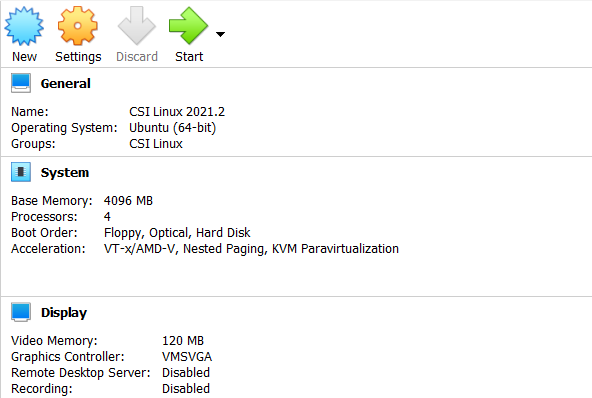
\includegraphics[height=7cm]{VirtualBox_1}
    \end{center}
\end{frame}

\begin{frame}{VirtualBox}
    1. Gebe Namen und Installationsort ein.\newline
    2. Unbeaufsichtigte Installation überspringen!
    \begin{center}
        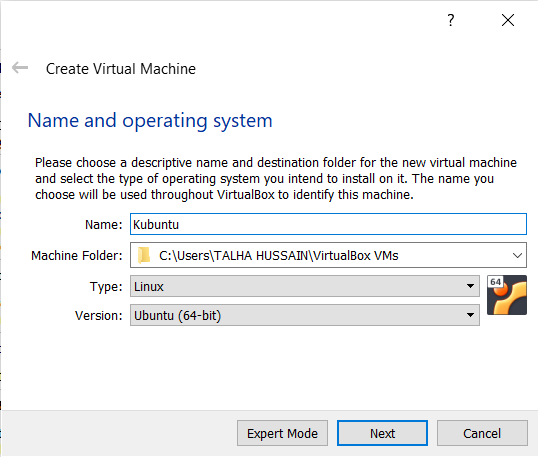
\includegraphics[height=6.5cm]{VirtualBox_2}
    \end{center}
\end{frame}

\begin{frame}{VirtualBox}
    \begin{center}
        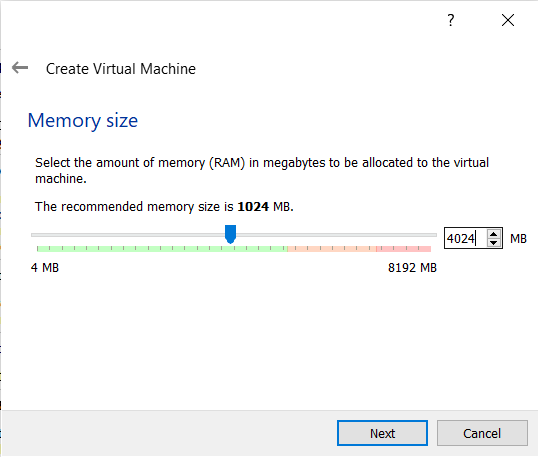
\includegraphics[height=7.5cm]{VirtualBox_3}
    \end{center}
\end{frame}

\begin{frame}{VirtualBox}
    \begin{center}
        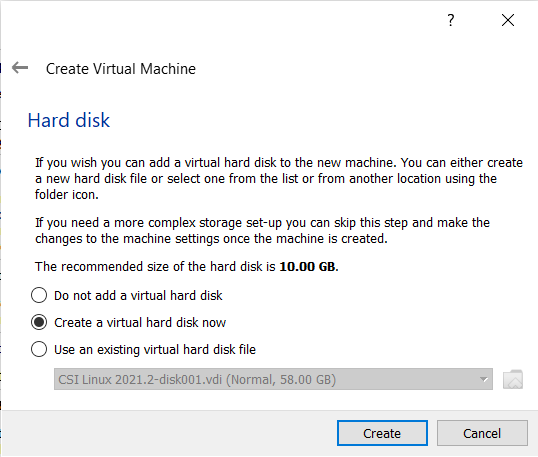
\includegraphics[height=7.5cm]{VirtualBox_4}
    \end{center}
\end{frame}

\begin{frame}{VirtualBox}
    Wähle VDI aus
    \begin{center}
        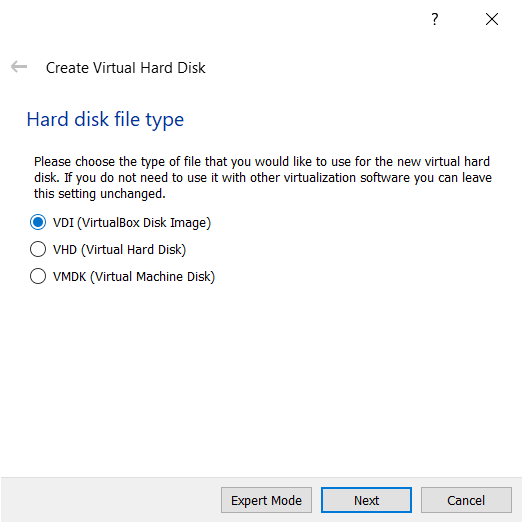
\includegraphics[height=7cm]{VirtualBox_5}
    \end{center}
\end{frame}

\begin{frame}{VirtualBox}
    \begin{center}
        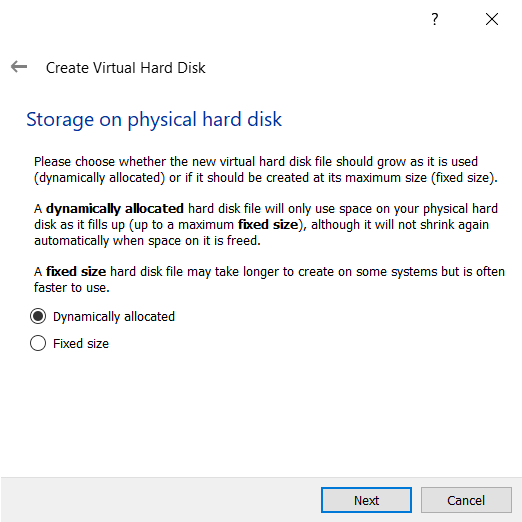
\includegraphics[height=7.5cm]{VirtualBox_6}
    \end{center}
\end{frame}

\begin{frame}{VirtualBox}
    Füge eine Virtuelle Festplatte mit 10-20GB hinzu.
    \begin{center}
        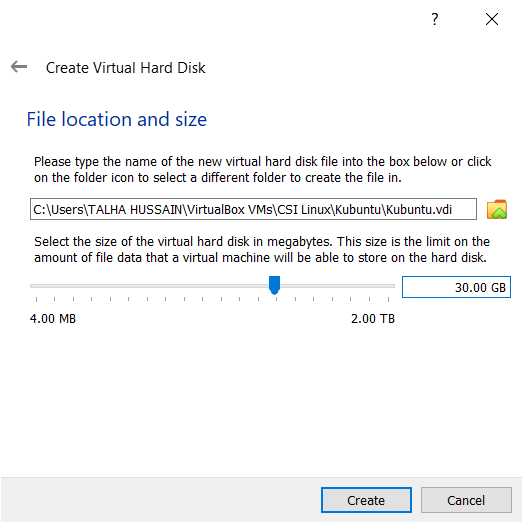
\includegraphics[height=7cm]{VirtualBox_7}
    \end{center}
\end{frame}

\begin{frame}{VirtualBox}
    Gehe in den Einstellungen der VM auf "Storage" und wähle die ISO-Datei aus.

    \begin{center}
        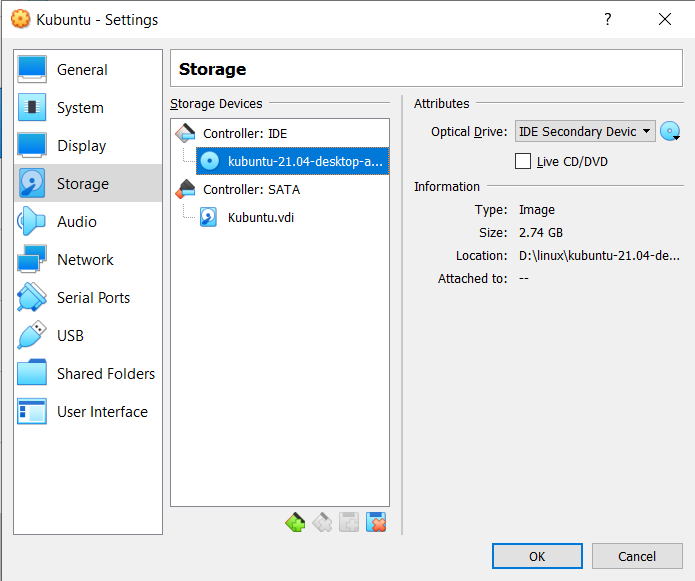
\includegraphics[height=6.5cm]{VirtualBox_8}
    \end{center}
\end{frame}

\begin{frame}{Einrichtung}
    \subsection{Einrichtung}\label{subsec:Einrichtung}
    Beginne den Install-Prozess mit dem Starten der VM und wähle "Kubuntu" aus.

    \begin{center}
        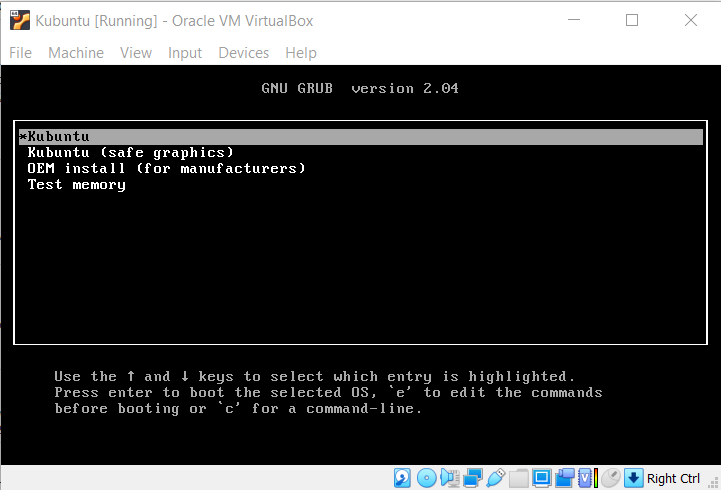
\includegraphics[height=6.5cm]{Install_1}
    \end{center}
\end{frame}

\begin{frame}{Einrichtung}
    Nach Starten des Live-Systems sind wir im grafischen Installer.
    \begin{center}
        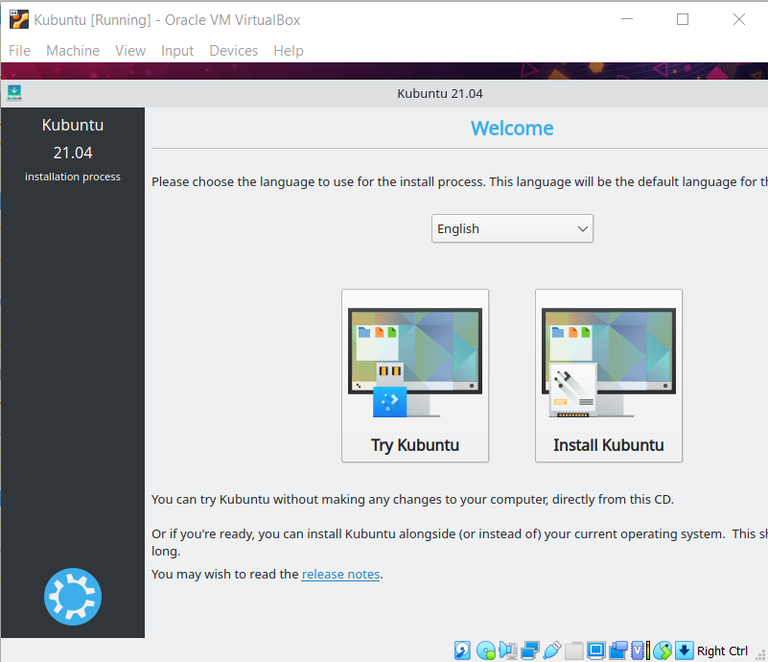
\includegraphics[height=6.5cm]{Install_2}
    \end{center}
\end{frame}

\begin{frame}{Einrichtung}
    Sprache: Deutsch
    \begin{center}
        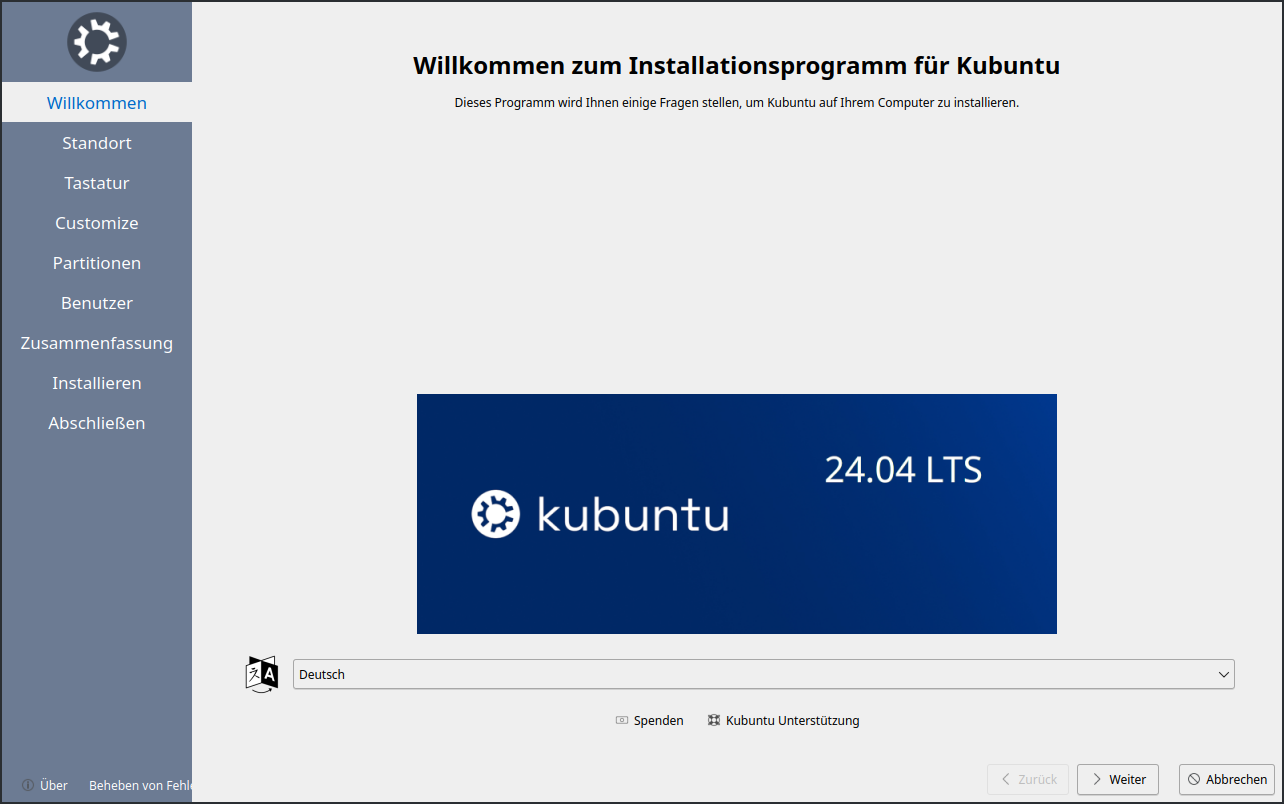
\includegraphics[height=6.5cm]{Install_3}
    \end{center}
\end{frame}

\begin{frame}{Einrichtung}
    Standort: Berlin
    \begin{center}
        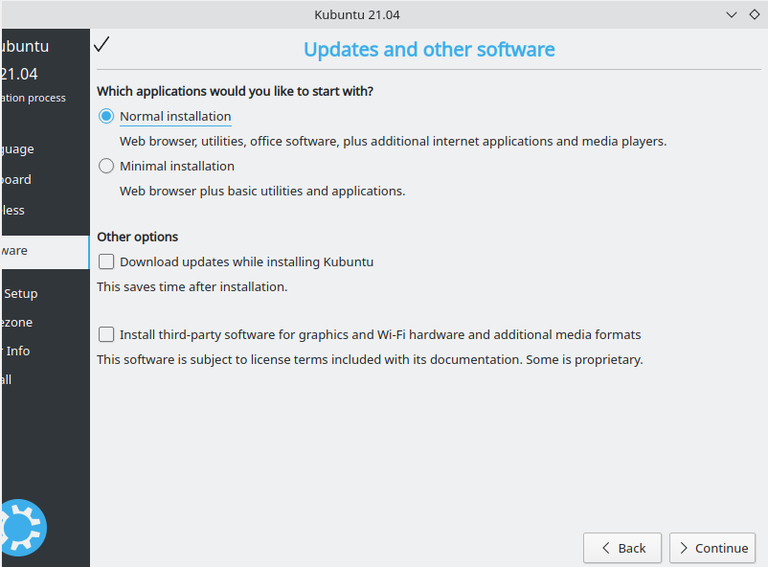
\includegraphics[height=6.5cm]{Install_4}
    \end{center}
\end{frame}

\begin{frame}{Einrichtung}
    Tastatur nach Wahl
    \begin{center}
        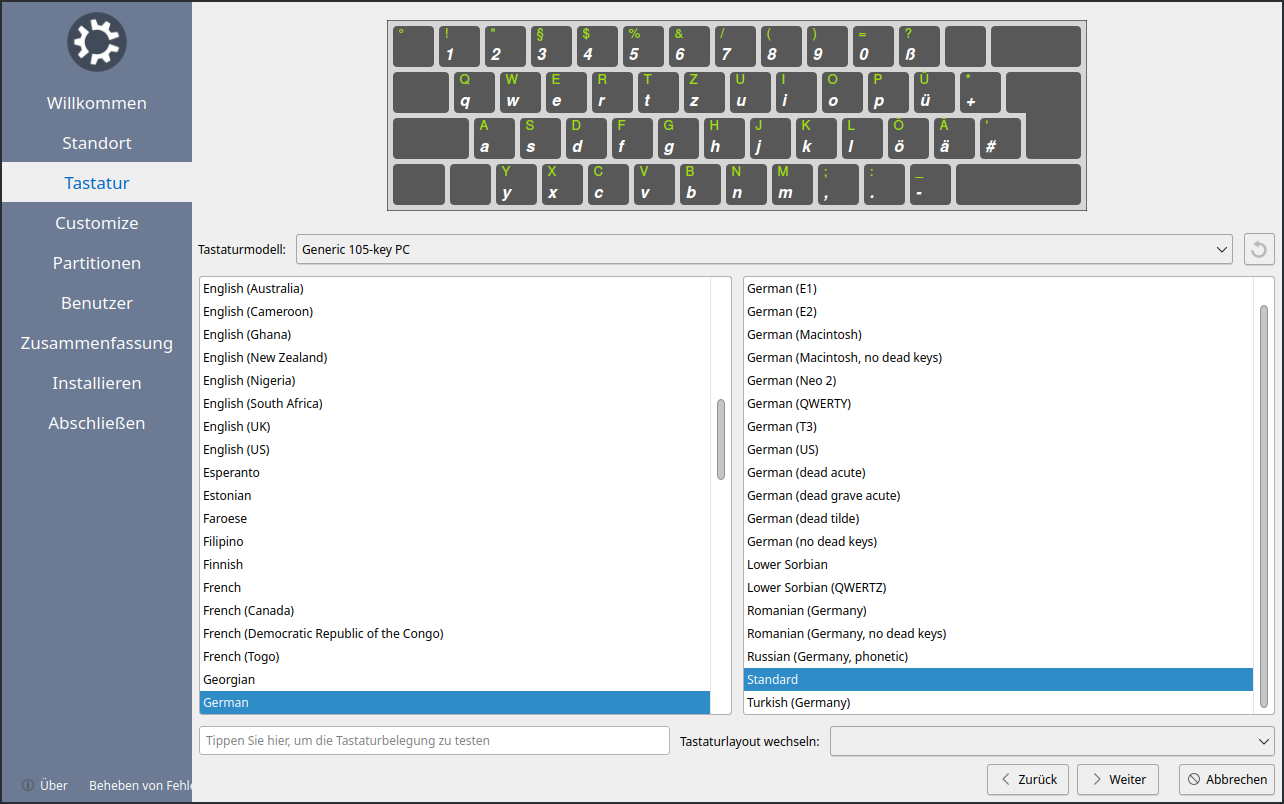
\includegraphics[height=6.5cm]{Install_5}
    \end{center}
\end{frame}

\begin{frame}{Einrichtung}
    Normale Installation
    \begin{center}
        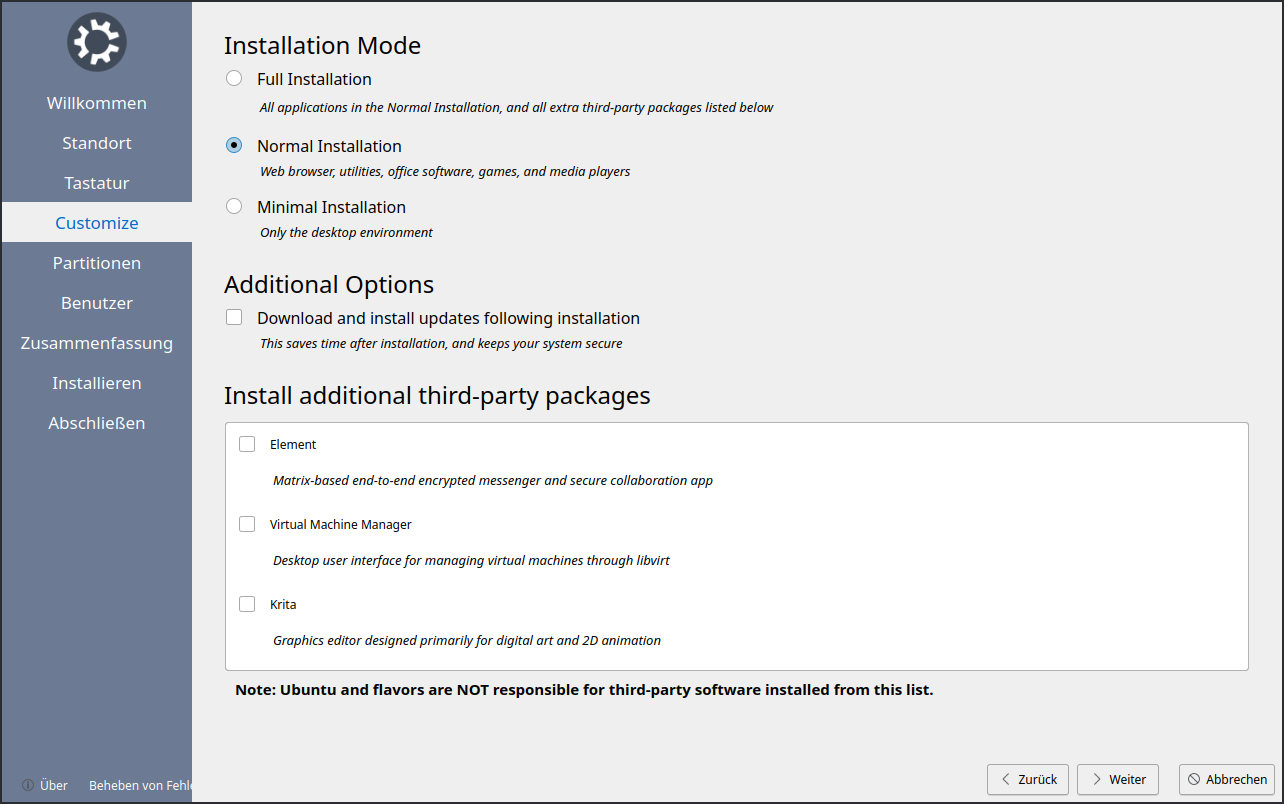
\includegraphics[height=6.5cm]{Install_6}
    \end{center}
\end{frame}

\begin{frame}{Einrichtung}
    "Festplatte Löschen" (Ganze virtuelle Festplatte)
    \begin{center}
        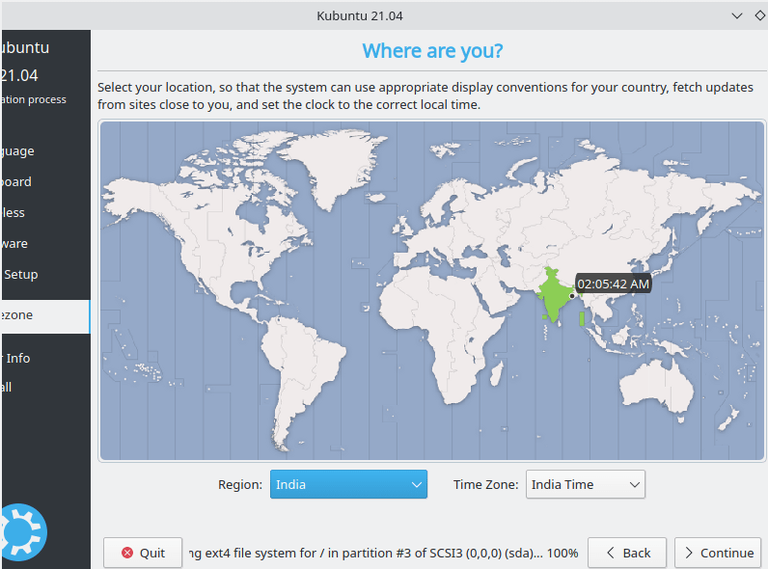
\includegraphics[height=6.5cm]{Install_7}
    \end{center}
\end{frame}

\begin{frame}{Einrichtung}
    Erstelle deinen Benutzer mit leichtem Passwort.
    \begin{center}
        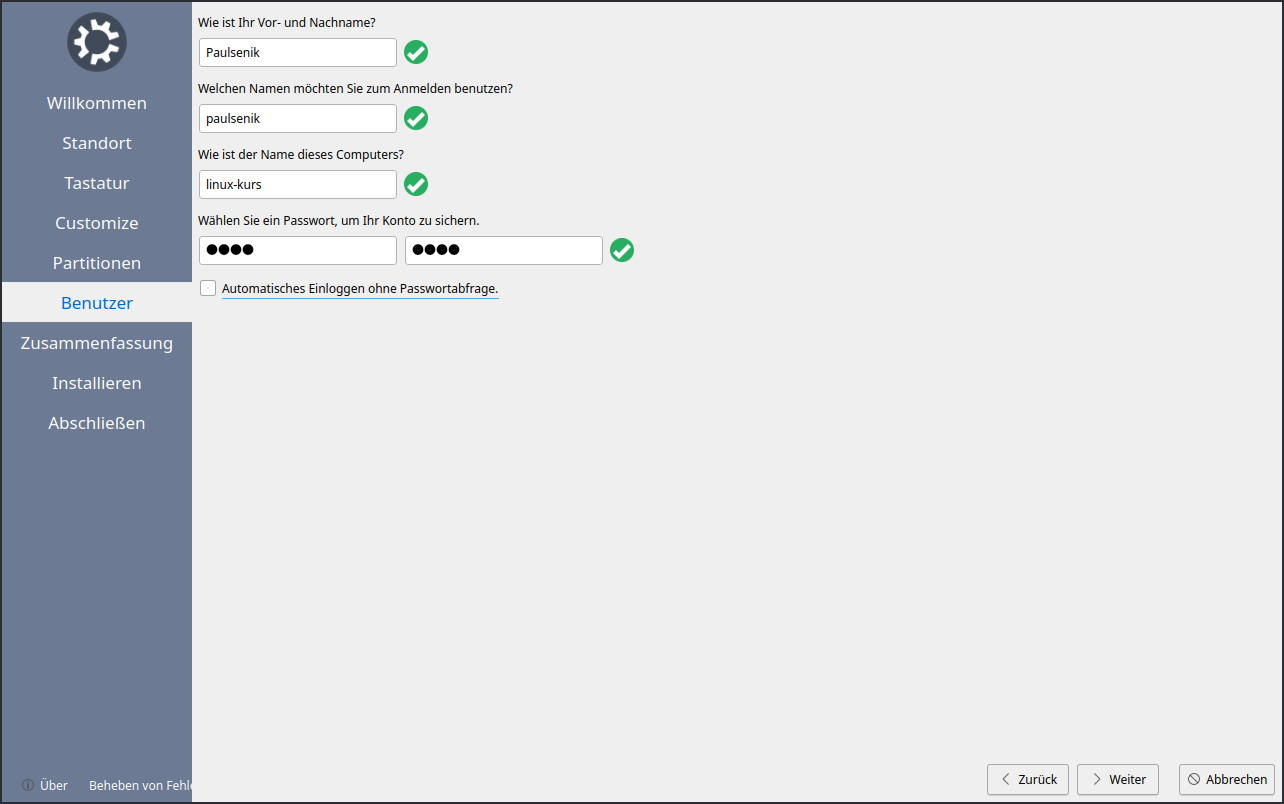
\includegraphics[height=6.5cm]{Install_8}
    \end{center}
\end{frame}

\begin{frame}{Einrichtung}
    Die Installationsübersicht
    \begin{center}
        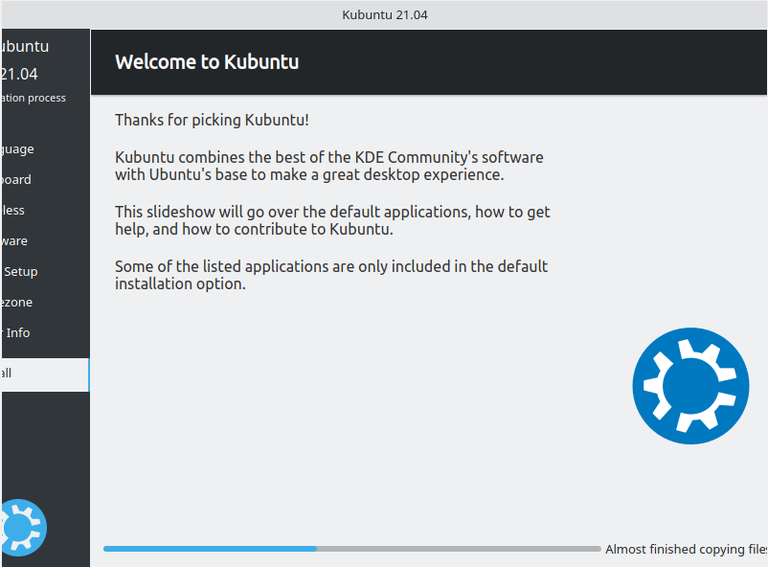
\includegraphics[height=6.5cm]{Install_9}
    \end{center}
\end{frame}

\begin{frame}{Einrichtung}
    Änderungen Bestätigen
    \begin{center}
        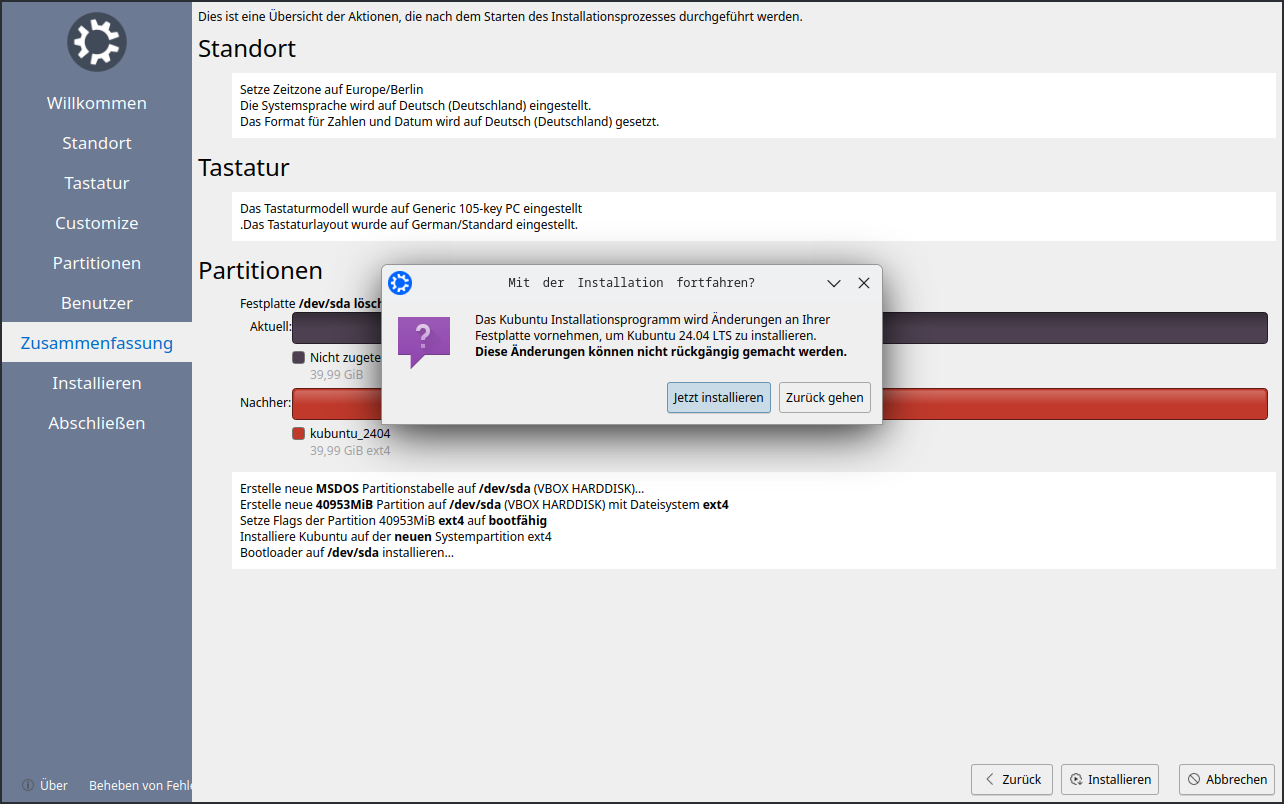
\includegraphics[height=6.5cm]{Install_10}
    \end{center}
\end{frame}

\begin{frame}{Einrichtung}
    Die Installation dauert etwas\dots
    \begin{center}
        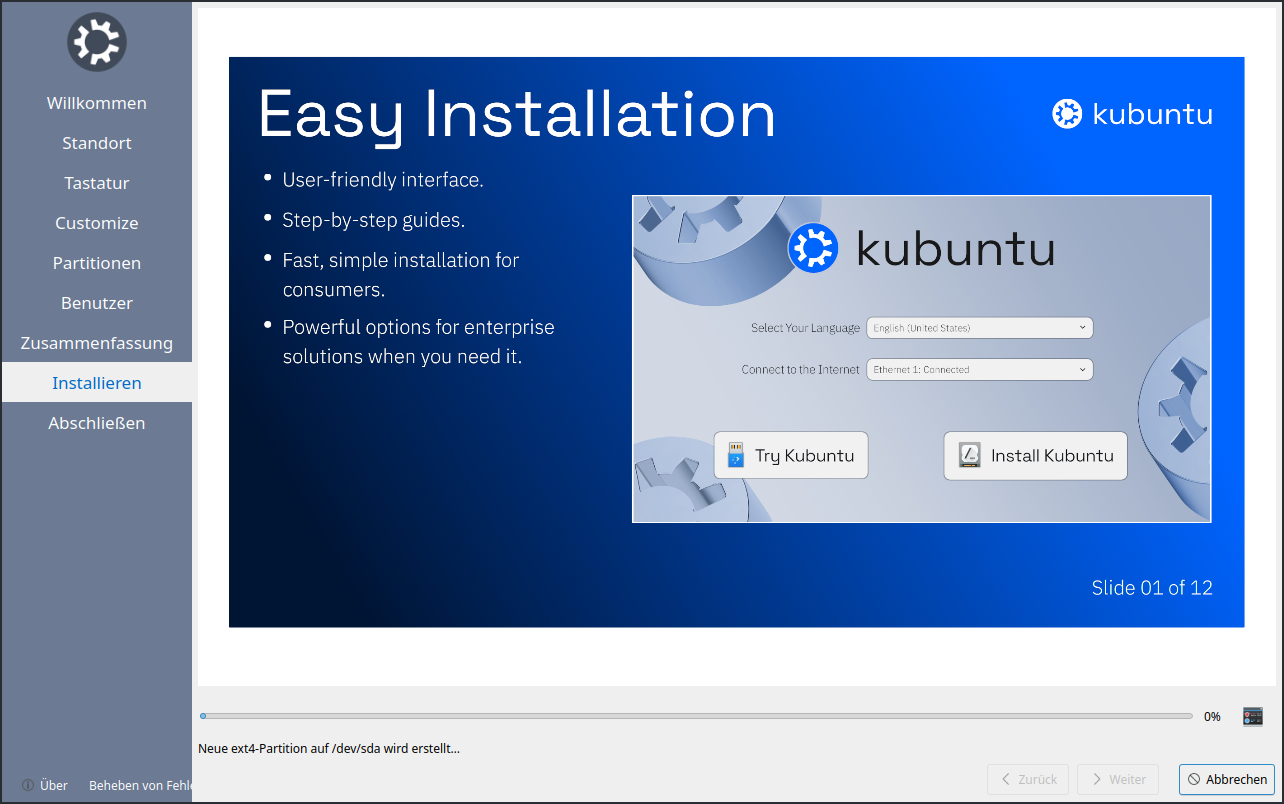
\includegraphics[height=6.5cm]{Install_11}
    \end{center}
\end{frame}

\begin{frame}{Einrichtung}
    Starte die VM nach Fertigstellung neu.
    \begin{center}
        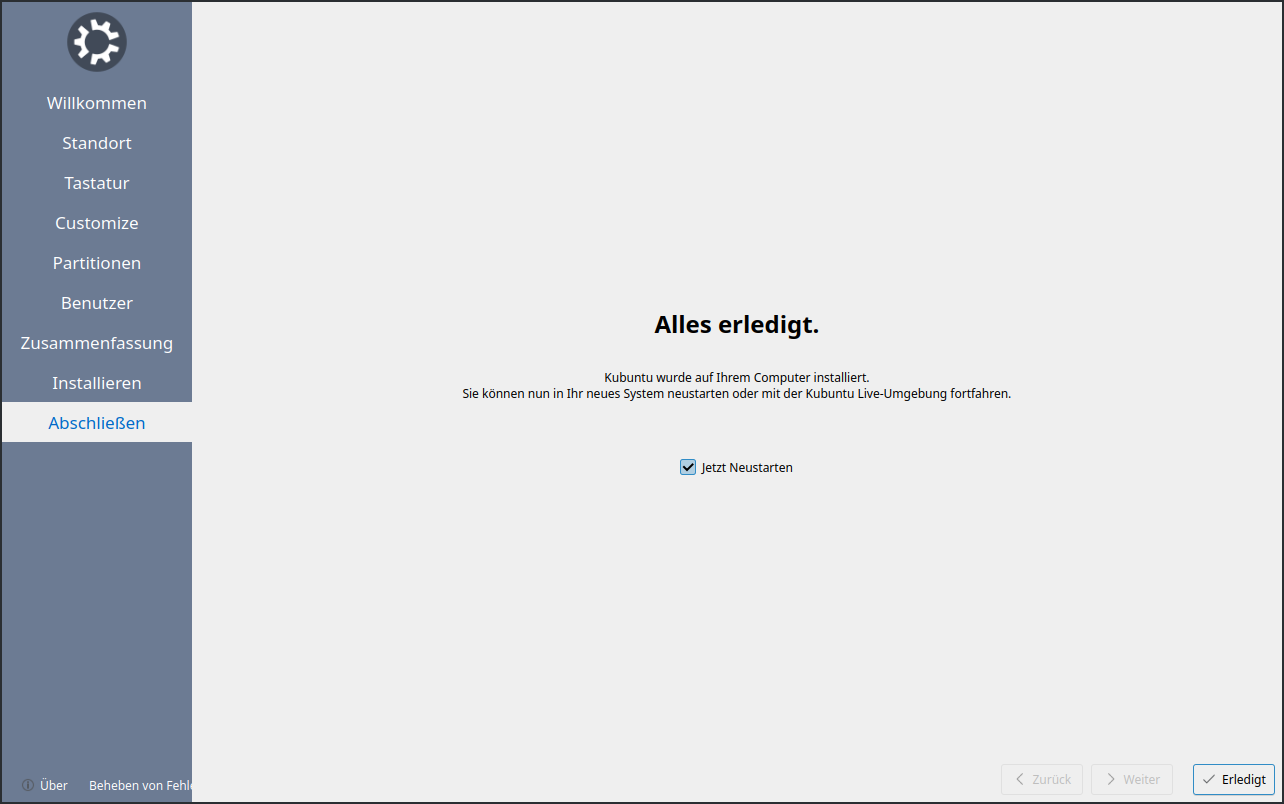
\includegraphics[height=6.5cm]{Install_12}
    \end{center}
\end{frame}

\begin{frame}{Einrichtung}
    Warte noch! Wir müssen die CD auswerfen!
    \begin{center}
        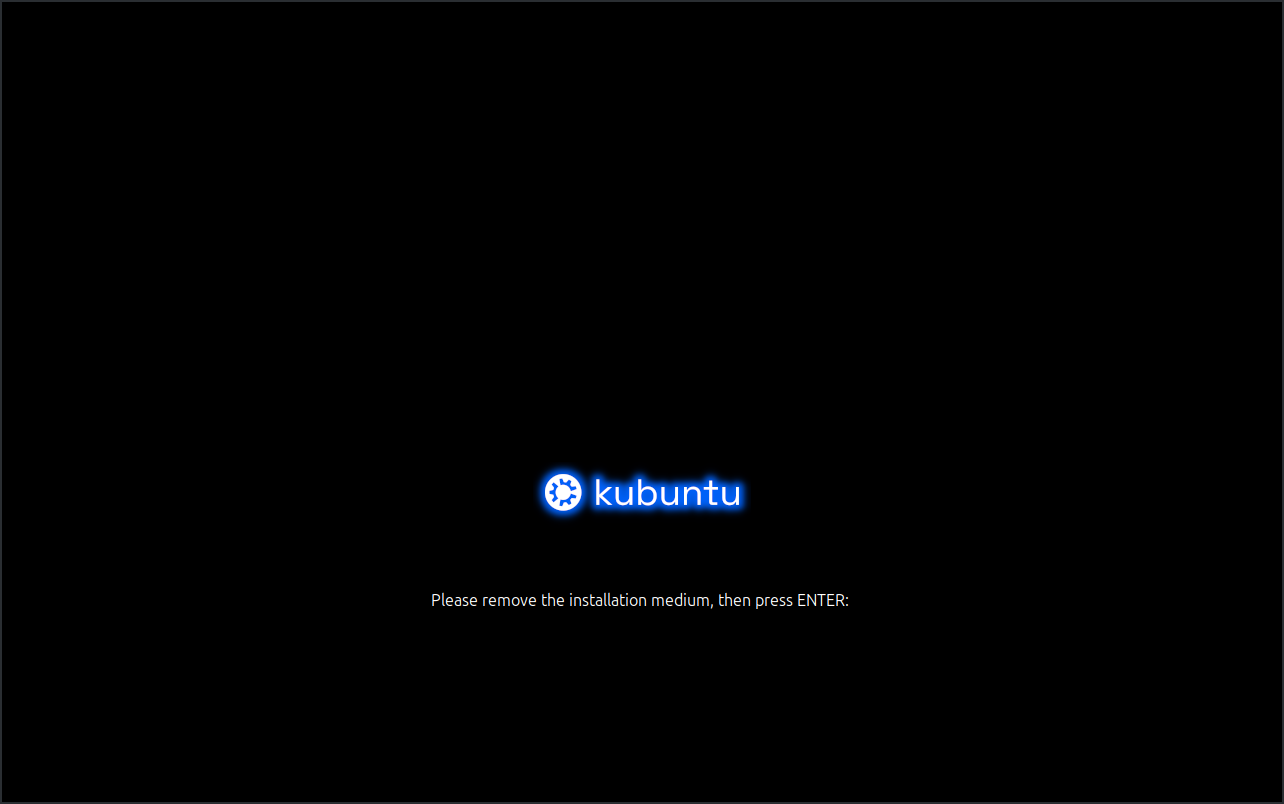
\includegraphics[height=6.5cm]{Install_13}
    \end{center}
\end{frame}

\begin{frame}{Einrichtung}
    Werfe die ISO-Datei aus!
    \begin{center}
        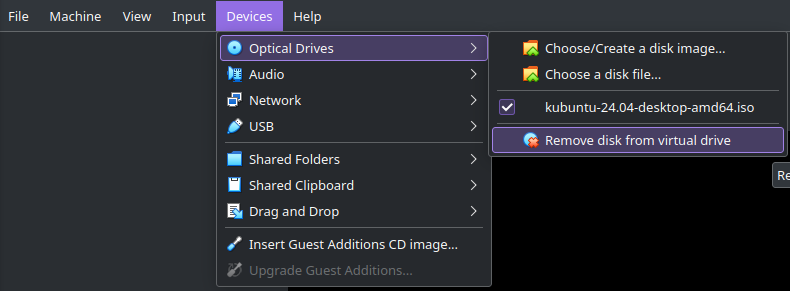
\includegraphics[width=10.5cm]{Install_14}
    \end{center}
    Drücke "Enter" im VM-Display und warte auf den kompletten Neustart!
\end{frame}